\documentclass{article}

% --- packages ---

\usepackage[utf8]{inputenc}
\usepackage[english, ngerman]{babel}
\usepackage{amsmath}
\usepackage{amsthm}
\usepackage{mathdots}
\usepackage[linesnumbered,ruled,noline]{algorithm2e}
\usepackage{tikz, pgfplots}
\usepackage{amssymb}
\usepackage{graphicx}
%\usepackage{subcaption}
\usepackage{pgf}
\usepackage{caption}
\usepackage{listings, lstautogobble}
\usepackage{delarray}
\usepackage{bigints}
\usepackage{float}
\usepackage{layouts}
\usepackage{subfigure}
\usepackage{url}
\usepackage{fancyhdr}
\usepackage{MnSymbol}
\usepackage{wasysym}
\usepackage[a]{esvect} %für bessere Vektorpfeile
\usepackage{setspace}
\usepackage{geometry}
\usepackage{hyperref}
\usepackage{booktabs}
\usepackage{array}
\usepackage{acronym}
\usepackage{ifsym}
\usepackage[sorting=nty]{biblatex}
\usepackage[nottoc,numbib]{tocbibind}

% --- Input macros von Ide ---

%\input{macros}

% --- Seitenränder / Einrücktiefe ---

\geometry{left=2.5cm, right=2.5cm, top=2cm, bottom=2cm}
\parindent0cm

% --- new commands ---

\newcommand{\RM}[1]{\MakeUppercase{\romannumeral #1{}}} %für römische Zahlen #1{}}} %für römische Zahlen
\newcommand{\xvec}{\underline{x}}
\newcommand{\bvec}{\underline{b}}
\newcommand{\uvec}{\underline{u}}
\newcommand{\vvec}{\underline{v}}
\newcommand{\wvec}{\underline{w}}
\newcommand{\pvec}{\underline{p}}
\newcommand{\zvec}{\underline{z}}
\newcommand{\xstern}{\underline{x}^*}
\newcommand{\Rmn}{\mathbb{R}^{m \times n}}
\newcommand{\Elasticsearch}{\textit{Elasticsearch}\;}
\newcommand{\Rnn}{\mathbb{R}^{n \times n}}
\newcommand{\rang}{\text{rang}}
\def\code#1{\texttt{#1}}
\newcommand{\dom}{\textrm{dom}}
\newcommand{\lojoin}{{\tiny \textifsym{d|><|}}}
\newcommand{\rojoin}{{\tiny \textifsym{|><|d}}}
\newcommand{\fojoin}{{\tiny \textifsym{d|><|d}}}
\newcommand{\m}{\cdot} %Malzeichen einfacher
\newcommand{\entspricht}{$\mathop{\hat{=}}$} %Entspricht-Zeichen
\renewcommand{\labelnamepunct}{\addcolon\space}

% -- Definitionen für Theoremumgebungen ---

\newtheoremstyle{newline}% name
{}% Space above
{\baselineskip}% Space below
{\normalfont}% Body font
{}% Indent amount
{\bfseries}% Theorem head font
{:}% Punctuation after theorem head
{\newline}% Space after theorem head
{\thmname{#1}\thmnumber{ #2}\thmnote{ (#3)}}% Theorem head spec (can be left empty, meaning ‘normal’ )

\theoremstyle{newline}
\newtheorem{definition}{Definition}[section]
\newtheorem{satz}[definition]{Satz}
\newtheorem{bemerkung}[definition]{Bemerkung}
\newtheorem{folgerung}[definition]{Folgerung}

\renewenvironment{proof}[1][\proofname:]{%
\minisec{#1}
\pushQED{\qed}%
\itshape
}{%
\popQED
\par
\medskip
}

% --- listing_settings ---
\lstset{
	language=Python,
	frame=single, % Rahmen um den Code
	numbers=left, % Zeilennummern auf der linken Seite
	numberstyle=\small, % Stil der Zeilennummern
	xleftmargin=2em, % Abstand zum linken Rand
	keywordstyle=\color{blue}, % Kewyord Style
	tabsize=4,
	breaklines=true,
}

% --- options for algorithm
\SetKwComment{Comment}{/* }{ */}


% --- Define colors ---

\definecolor{red}{rgb}{0.6,0,0} % for strings
\definecolor{blue}{rgb}{0,0,0.6}
\definecolor{green}{rgb}{0,0.8,0}
\definecolor{cyan}{rgb}{0.0,0.6,0.6}
\newcommand{\greencomment}[1]{\textcolor{green}{#1}}


\lstset{autogobble=true}

% --- Literaturverzeichnis ---


% --- Beginn des eigentlichen Dokuments ---


\begin{document}

% -- Layout Kopfzeile ---

\pagestyle{fancy}
\lhead{\small{\slshape}}
\chead{}	
\rhead{\mdseries \leftmark}


\begin{titlepage}

%\includegraphics[width=0.20\textwidth]{Bilder/fh_logo.png}\hfill\includegraphics[width=0.25\textwidth]{Bilder/diamant-software-logo-teams.png}

% --- include correct images here

\centering

{\bfseries HSBI Bielefeld \par}
\vspace{0.25cm}
{\bfseries University of Applied Sciences \par}
\vspace{0.25cm}
{\bfseries Fachbereich Ingenieurwissenschaften und Mathematik \par}
\vspace{0.25cm}
{\bfseries Studiengang Optimierung und Simulation \par}
\vspace{1.5cm}
{\huge\bfseries Lösen von nichtlinearen Gleichungssystemen mit einem Reinforcement-Learning-Agent \par}
\vspace{2.5cm}
{\Large\bfseries Bericht \par}
{\vspace{8.5cm}}

\flushleft
\begin{tabular}{ll}
	Vorgelegt von: & Nicolas Schneider \vspace{0.25cm}\\
	Matrikelnummer: & 1208960 \vspace{0.25cm} \\
	Studiengang: & Optimierung und Simulation \vspace{0.5cm} \\
	Abgabedatum: & 07.04.2024 \vspace{0.5cm} \\
	Betreuer: & Prof. Dr. rer. nat. Bernhard Bachmann
\end{tabular}
\vfill
\end{titlepage}


\thispagestyle{empty}
\newpage



\begin{onehalfspace}

\thispagestyle{empty}
\selectlanguage{english}
\begin{abstract}
	Nichtlineare Gleichungssysteme (NGS) spielen eine zentrale Rolle in vielen Bereichen der Wissenschaft und Technik, da sie zur Modellierung und Lösung komplexer Probleme in Physik, Chemie, Ingenieurwesen und anderen Disziplinen eingesetzt werden. Trotz ihrer Bedeutung stellt die Lösung von NGS aufgrund ihrer inhärenten Nichtlinearität und des Fehlens geschlossener analytischer Lösungen eine große Herausforderung dar. Traditionelle numerische Verfahren wie das Newton-Raphson-Verfahren oder Optimierungsansätze stoßen oft an ihre Grenzen, insbesondere bei hochdimensionalen Problemen, chaotischem Verhalten oder starker Abhängigkeit von Anfangsbedingungen.
	
	In jüngster Zeit hat der Bereich des Reinforcement Learnings (RL) zunehmend an Bedeutung gewonnen und vielversprechende Ergebnisse bei der Lösung komplexer Probleme geliefert. RL-Agenten lernen durch Interaktion mit einer Umgebung und Belohnungssignale, optimale Strategien zu entwickeln, ohne explizite Programmierung. Dieser Ansatz hat sich in verschiedenen Anwendungsfeldern wie Robotik, Spielen und Optimierungsproblemen als erfolgreich erwiesen.
	\\
	
	In dieser Arbeit werden die beiden Ansätze der nichtlinearen Gleichungssysteme kombiniert, wobei ein Fokus auf die Integration von Reinforcement Learning (RL) liegt, um Lösungen zu generieren. Ein RL-Agent wird in einer maßgeschneiderten Umgebung trainiert, die die Struktur des gegebenen nichtlinearen Gleichungssystems widerspiegelt. Durch die Formulierung von Belohnungen für Aktionen, die den Agenten näher an eine Lösung führen, wird dieser befähigt, iterative Strategien zur effizienten Lösungsfindung zu erlernen.
	
	Die vorliegende Arbeit präsentiert einen initiierenden Ansatz und analysiert seine Leistung hinsichtlich Schnelligkeit und Genauigkeit bei der Lösungsfindung von nichtlinearen Gleichungssystemen. Dabei wird eine eingehende Untersuchung durchgeführt, um die Effektivität dieses Ansatzes im Vergleich zu etablierten Methoden wie dem Newton-Raphson-Verfahren zu bewerten. Besonderes Augenmerk wird auf die Identifizierung und Analyse der limitierenden Faktoren dieses Ansatzes gelegt, um potenzielle Schwächen aufzudecken und zu verstehen, inwiefern dieser Ansatz für praktische Anwendungen geeignet ist.
	
	% Hier noch Ergebnisse kurz darstellen?
	
\end{abstract}
\selectlanguage{ngerman}
\newpage


\tableofcontents	% Inhaltsverzeichnis		
\thispagestyle{empty}

\newpage		

\section{Grundlagen nichtlinearer Gleichungssysteme}

Ein nichtlineares Gleichungssystem kann als Nullstellenproblem wie folgt formuliert werden:

\begin{definition}[Nichtlineares Gleichungssystem]
	Es sei $B \subset \mathbb{R}^n$ und $\mathbf{g}: B \rightarrow \mathbb{R}^n$. Gesucht sind Lösungen von
	
	\begin{center}
		$\mathbf{f}(\mathbf{x}) = \mathbf{0}.$
	\end{center}
	
	$\mathbf{f}(\mathbf{x}) = \mathbf{0}$ ist ein System von $n$ nichtlinearen Gleichungen für $n$ Unbekannte $x_1, \dots, x_n$.
	\\
	
	\begin{center}
		\boxed{
			\begin{array}{ccc}
				f_1(x_1, \dots, x_n) & = &0\\
				f_2(x_1, \dots, x_n) & = & 0\\
				\vdots &&\\
				f_n(x_1, \dots, x_n) & = & 0
			\end{array}
		}
	\end{center}
	
\end{definition}
\bigskip

Nichtlineare Gleichungssysteme treten in vielen Bereichen der Wissenschaft und Technik auf, wie beispielsweise in der Physik, Chemie, Biologie, Wirtschaftswissenschaften und Ingenieurwissenschaften. Sie dienen zur Modellierung und Analyse komplexer Systeme, deren Verhalten durch nichtlineare Beziehungen zwischen den Variablen beschrieben wird.

Die Lösung solcher Systeme ist jedoch oft eine große Herausforderung, da nichtlineare Gleichungen im Allgemeinen keine geschlossenen analytischen Lösungen besitzen. Stattdessen müssen numerische Verfahren eingesetzt werden, um approximative Lösungen zu finden. Einige gängige Methoden zur Lösung nichtlinearer Gleichungssysteme sind:

\begin{enumerate}
	\item \textbf{Iterative Verfahren}: Hierzu zählen Methoden wie das Newton-Verfahren, das Quasi-Newton-Verfahren und das Broyden-Verfahren. Diese Verfahren starten mit einer Anfangsschätzung und verbessern diese iterativ, bis eine ausreichend genaue Lösung gefunden ist.
	
	\item \textbf{Globale Optimierungsverfahren}: Wenn das Gleichungssystem als Optimierungsproblem formuliert werden kann, können globale Optimierungsverfahren wie die Branch-and-Bound-Methode oder evolutionäre Algorithmen zur Lösung eingesetzt werden.
\end{enumerate}

Die Schwierigkeit, nichtlineare Gleichungssysteme zu lösen, besteht oft darin, geeignete Anfangsschätzungen für die Iterationsverfahren zu finden und die Konvergenz der Verfahren sicherzustellen. Viele Systeme weisen mehrere Lösungen auf, von denen einige instabil oder nicht physikalisch sinnvoll sein können. Darüber hinaus können nichtlineare Systeme eine komplexe Struktur mit mehreren lokalen Extrema aufweisen, was die globale Konvergenz erschwert. 


\section{Grundlagen Reinforcement Learning}

Reinforcement Learning (RL) ist ein Teilgebiet des Maschinellen Lernens, bei dem ein Agent lernt, durch Interaktion mit einer Umgebung eine bestimmte Aufgabe oder ein Ziel zu erreichen. Im Gegensatz zu überwachtem Lernen, bei dem ein Modell anhand von Trainingsbeispielen mit bekannten Eingabe-Ausgabe-Paaren gelernt wird, erhält der Agent beim Reinforcement Learning nur eine skalare Bewertung (Reward) für seine Aktionen. Durch Ausprobieren und Lernen aus den erhaltenen Rewards versucht der Agent, eine Strategie (Policy) zu finden, die die kumulative Belohnung über die Zeit maximiert.
\\

\textbf{Markov-Entscheidungsprozess:}
\smallskip

Reinforcement Learning Probleme werden häufig als Markov-Entscheidungsprozesse (Markov Decision Processes, MDPs) formuliert. Ein MDP besteht aus:

\begin{itemize}
	\item Einem Zustandsraum $\mathcal{S}$, der alle möglichen Zustände der Umgebung enthält.
	\item Einem Aktionsraum $\mathcal{A}$, der alle möglichen Aktionen des Agenten definiert.
	\item Einer Übergangswahrscheinlichkeitsfunktion $\mathcal{P}(s, a, s')$, die die Wahrscheinlichkeit angibt, dass der Agent beim Ausführen der Aktion $a$ im Zustand $s$ in den Zustand $s'$ übergeht.
	\item Einer Belohnungsfunktion $\mathcal{R}(s, a, s')$, die die Belohnung definiert, die der Agent erhält, wenn er aus dem Zustand $s$ durch Ausführen der Aktion $a$ in den Zustand $s'$ übergeht.
\end{itemize}

Das Ziel des Agenten ist es, eine Policy $\pi: \mathcal{S} \rightarrow \mathcal{A}$ zu finden, die die erwartete kumulative Belohnung über die Zeit maximiert.

Abbildung \ref{fig:rl_grundlagen} stellt den Lernprozess eines Agenten in einer Umgebung vereinfacht dar.

\begin{figure}[h]
	\centering
	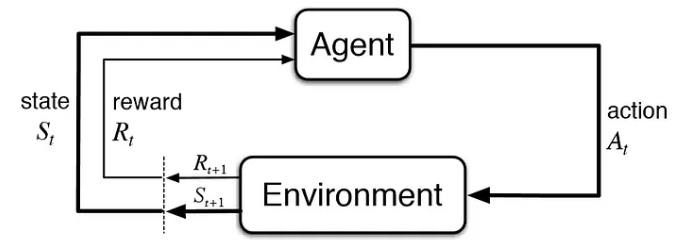
\includegraphics[width=0.5\textwidth]{Bilder/rl_grundlagen.png}
	\caption{Vereinfachter Lernprozess eines Agenten in einer Umgebung\protect\footnotemark}
	\label{fig:rl_grundlagen}
\end{figure}
\footnotetext{\url{https://towardsdatascience.com/reinforcement-learning-101-e24b50e1d292}}


\textbf{Value Functions und Bellman-Gleichungen:}
\smallskip

Eine zentrale Rolle beim Reinforcement Learning spielen die Value Functions, die den erwarteten kumulativen Reward für einen gegebenen Zustand oder eine Zustand-Aktions-Paar angeben. Es gibt zwei wichtige Value Functions:

\begin{itemize}
	\item Die State-Value Function $V^\pi(s)$ gibt den erwarteten kumulativen Reward an, wenn der Agent im Zustand $s$ startet und der Policy $\pi$ folgt.
	\item Die Action-Value Function $Q^\pi(s, a)$ gibt den erwarteten kumulativen Reward an, wenn der Agent im Zustand $s$ startet, die Aktion $a$ ausführt und danach der Policy $\pi$ folgt.
\end{itemize}

Die Value Functions erfüllen die Bellman-Gleichungen, die eine rekursive Beziehung zwischen den Value Functions benachbarter Zustände herstellen. Für die State-Value Function lautet die Bellman-Gleichung:

\begin{equation}
	V^\pi(s) = \mathbb{E}_\pi \left[ R(s, a, s') + \gamma V^\pi(s') \right]
\end{equation}

Und für die Action-Value Function:

\begin{equation}
	Q^\pi(s, a) = \mathbb{E}_\pi \left[ R(s, a, s') + \gamma \sum_{s'} \mathcal{P}(s, a, s') V^\pi(s') \right]
\end{equation}

Hier ist $\gamma \in [0, 1]$ der Diskontierungsfaktor, der bestimmt, wie viel Gewicht zukünftigen Rewards beigemessen wird. Ein Wert von $\gamma$ nahe 0 bedeutet, dass der Agent nur die unmittelbaren Rewards optimiert, während ein Wert nahe 1 längerfristige Belohnungen stärker gewichtet.
\\

\textbf{Proximal Policy Algorithmus (PPO):}
\smallskip

Proximal Policy Optimization (PPO) ist ein moderner Algorithmus im Bereich des Reinforcement Learning, der zur Klasse der Policy Gradient Methoden gehört. PPO wurde von Schulman et al. \cite{schulman2017proximal} entwickelt und hat sich aufgrund seiner guten Performanz und Stabilität in verschiedenen Anwendungsbereichen etabliert.
\medskip

Das Ziel von PPO ist es, eine optimale Policy zu finden, die die erwartete kumulative Belohnung maximiert. Im Gegensatz zu klassischen Policy Gradient Methoden, die oft große Schritte im Parameterraum machen und dadurch instabil werden können, verwendet PPO eine Clipping-Technik, um die Größe der Policy-Updates zu begrenzen. Dadurch wird eine stabilere Konvergenz erreicht und die Wahrscheinlichkeit von Divergenz oder schlechten Performanz reduziert.
\medskip

Der Kerngedanke von PPO besteht darin, die Policy-Updates so zu gestalten, dass sie innerhalb einer vertrauenswürdigen Region (trust region) bleiben. Dies wird erreicht, indem die Differenz zwischen der alten und der neuen Policy durch eine Clipping-Funktion begrenzt wird. Die Clipping-Funktion schneidet die Wahrscheinlichkeitsverhältnisse (probability ratios) zwischen der alten und der neuen Policy bei vordefinierten Schwellenwerten ab.
\medskip

Formal lässt sich die Zielfunktion von PPO wie folgt darstellen:

\begin{equation}
	L^{CLIP}(\theta) = \hat{\mathbb{E}}_t \left[ \min(r_t(\theta)\hat{A}_t, \text{clip}(r_t(\theta), 1-\epsilon, 1+\epsilon)\hat{A}_t) \right]
\end{equation}

Hierbei ist $\theta$ der Parametervektor der Policy, $r_t(\theta) = \frac{\pi_\theta(a_t|s_t)}{\pi_{\theta_{old}}(a_t|s_t)}$ das Wahrscheinlichkeitsverhältnis zwischen der neuen und der alten Policy, $\hat{A}_t$ der geschätzte Vorteil und $\epsilon$ ein Hyperparameter, der die Größe der vertrauenswürdigen Region steuert.
\medskip

Der Term $\min(r_t(\theta)\hat{A}_t, \text{clip}(r_t(\theta), 1-\epsilon, 1+\epsilon)\hat{A}_t)$ sorgt dafür, dass die Policy-Updates innerhalb der vertrauenswürdigen Region bleiben. Wenn das Wahrscheinlichkeitsverhältnis $r_t(\theta)$ außerhalb des Intervalls $[1-\epsilon, 1+\epsilon]$ liegt, wird es auf die Grenzen des Intervalls gesetzt. Dadurch werden zu große Policy-Updates vermieden und die Stabilität des Lernprozesses verbessert.
\medskip

PPO verwendet häufig auch eine Value Function $V_\phi(s)$, um den Wert eines Zustands zu schätzen. Die Value Function wird verwendet, um den Vorteil $\hat{A}_t$ zu berechnen, der die Qualität einer Aktion im Vergleich zum erwarteten Wert des Zustands angibt. Der Vorteil kann beispielsweise durch die Generalized Advantage Estimation (GAE) \cite{schulman2015high} geschätzt werden.
\medskip

Insgesamt bietet PPO eine effektive und stabile Methode zum Lernen von Policies in Reinforcement Learning Problemen. Durch die Verwendung der Clipping-Technik und der vertrauenswürdigen Region werden große Policy-Updates vermieden und eine stabile Konvergenz erreicht. PPO hat sich in verschiedenen Benchmark-Problemen und realen Anwendungen bewährt und ist ein weit verbreiteter Algorithmus im Bereich des Reinforcement Learning.
\\

Neben dem Proximal-Policy-Algorithmus gibt es noch eine Vielzahl weiterer Algorithmen, die sich über die Zeit entwickelt haben, wie bspw. dem \textit{Deep Deterministic Policy Gradient} (DDPG)-, \textit{Twin Delayed DDPG} (TD3)-, oder dem \textit{Soft Actor Critic}-Algorithmus (SAC).
\\

Dieses Kapitel bietet lediglich einen grundlegenden Einblick in die Arbeitsweise des Reinforcement Learning. Es ist wichtig zu betonen, dass die konkrete Umsetzung eines Reinforcement-Learning-Agenten stark vom spezifischen Anwendungsfall und den zugrunde liegenden Daten und Informationen abhängt. Da Reinforcement Learning äußerst flexibel und anpassungsfähig ist, kann die Implementierung eines RL-Agenten in verschiedenen Szenarien und Kontexten erheblich variieren. 

\section{Reinforcement Learning für die Lösung nichtlinearer Gleichungssysteme}

Bevor ein RL-Agent nichtlineare Gleichungssysteme lösen kann, sollten zunächst einige wichtige Fragen beantwortet werden, die für die Qualität der Lösung und die Lösungsfindung von Relevanz sind:

\begin{enumerate}
	\item \textbf{Umgebung:} Was ist die Umgebung, in dem der Agent agiert?
	\item \textbf{Zustand:} Was sind zulässige und sinnvolle Zustände?
	\item \textbf{Aktionen:} Was sind zulässige und sinnvolle Aktionen, die der Agent wählen kann?
	\item \textbf{Belohnung:} Wie sieht eine zielführende Belohnungsfunktion aus?
\end{enumerate}

Diese Projektarbeit fokussiert sich auf einen Teil der potenziellen Antworten auf die genannten Fragen. Es sei jedoch angemerkt, dass es alternative Formulierungen geben könnte, die ebenfalls zu einer effektiven Lösung beitragen können.
\\

\underline{Umgebung:}
\smallskip

Im Kontext dieses Projekts wird die Umgebung als der Raum betrachtet, in dem sich die Gleichungen befinden. Die Besonderheit dabei ist, dass, sollten die Gleichungen sich im Verlauf der Lösungsfindung nicht ändern, die Umgebung statisch ist. 
\\

\underline{Zustand:}
\smallskip

Der Zustand wird aufgefasst, als die gewählte Aktion.
\\

\underline{Aktion:}
\smallskip

Abhängig von der Dimensionalität des Problems kann der Agent aus einem kontinuierlichen Raum von Punkten wählen. Der Agent wählt eine Aktion $a \in \mathcal{A}$, wobei $\mathcal{A} \subseteq \mathbb{R}^{n-1}$ und $n$ die Dimensionalität des Problems widerspiegelt.
\\
 
\underline{Belohnungsfunktion:}
\smallskip

Die Formulierung der Belohnungsfunktion konzentriert sich darauf, die Lösung(en) des Gleichungssystem(s) zu finden, sofern sie denn existieren. In dieser Arbeit wird das Residuum verwendet, welches den Fehler zur eigentlichen Lösung darstellt. Das Residuum $R$ an der Optimallösung $x^{\ast}$ ist $0$, sodass das Ziel dabei ist diesen Fehler zu minimieren. 

\begin{definition}[Residuum]
	Gegeben seien $n$ nichtlineare Gleichungen mit $\mathbb{R}^n \rightarrow \mathbb{R}^n$. Es sei vorausgesetzt, dass mindestens eine Lösung $\mathbf{x}^{\ast}$ existiert, die das Gleichungssystem löst. Dann ist das Residuum an der Stelle $\mathbf{x}$ mit $\mathbf{x} \in \mathbb{R}^n$ definiert als
	
	\begin{equation}
		R(\mathbf{x}) = \sum\limits (f_i(\mathbf{x}) - f_j(\mathbf{x}))^2 \quad \forall 1 \leq i < j \leq n.
	\end{equation}
\end{definition}

Da der Agent das Ziel verfolgt die Belohnung über die Zeit zu maximieren, kann das negative Residuum als Belohnung interpretiert werden. $Reward = -R(\mathbf{x})$.
\\

Dieses Kapitel stellt die verfolgten Ansätze dar, die bei der Umsetzung verfolgt wurden. Im folgenden Kapitel wird genauer auf die Umsetzung dieses Ansatzes eingegangen.

\section{Umsetzung}

Bevor mit der Implementierung der Problemstellung, der Umgebung und des Agents begonnen wird, ist es von entscheidender Bedeutung, die Auswahl der richtigen Programmiersprache und Bibliothek sorgfältig zu prüfen. Diese Entscheidung bildet das Fundament für das gesamte Projekt und kann einen erheblichen Einfluss auf die Effizienz, Skalierbarkeit und den Erfolg der Umsetzung haben.
\medskip

Für dieses Projekt wurde die Programmiersprache \textit{Python} als Programmiersprache gewählt, zusammen mit der Reinforcement-Learning-Bibliothek \textit{stable-baselines3}. Diese Entscheidung basiert darauf, dass \textit{stable-baselines3} eine breite Palette von wichtigen RL-Algorithmen implementiert und gleichzeitig eine benutzerfreundliche Integration mit \textit{Python} bietet. Außerdem bietet diese Bibliothek eine ausgezeichnete Kompatibilität mit der Programm-Bibliothek \textit{gymnasium} von OpenAI, die essensziell für Erstellung von RL-Umgebungen ist. Die Kombination aus \textit{Python}, \textit{stable-baselines3} und \textit{gymnasium} ermöglicht eine effiziente Entwicklung und Umsetzung von Reinforcement-Learning-Algorithmen für die gegebenen Anforderungen des Projekts.
\\

Für die Umsetzung des Agenten bzw. der Umgebung sind folgende Methoden für die Problemstellung relevant:

\begin{itemize}
	\item \textbf{\code{get\_distance(x)}}: Berechnet das Residuum für einen Vektor $\mathbf{x} \in \mathbb{R}^{n-1}$.
	\item \textbf{\code{reward(residuum, *args)}}: Berechnet den Reward basierend auf dem Residuum und weiteren zusätzlichen Parametern.
	\item \textbf{\code{step(action)}}: Führt einen Schritt während des Lernens in der Umgebung aus und aktualisiert dabei die Belohnung auf Grundlage verschiedener, vorher festgelegter Regeln.
	\item \textbf{\code{reset()}}: Setzt die Umgebung auf einen zufälligen Zustand zurück.
\end{itemize}
\bigskip

\underline{Nichtlineares Gleichungssystem:}
\smallskip

Das nichtlineare Gleichungssystem kann mit einfachen Python-Funktionen umgesetzt werden. Nachfolgend ist ein Bespiel für eine Variante der Rosenbrock-Funktion angegeben, wie sie im Projekt-Code umgesetzt ist.

\begin{lstlisting}[language=Python, caption={Nichtlineares Gleichungssystem in Python}, label={lst:python}]
	def nse():
		eq1 = lambda x: 10 * (x[1] - x[0] ** 2)
		eq2 = lambda x: 1 - x[0]
	
	return [eq1, eq2]
\end{lstlisting}

Das Gleichungssystem kann dabei mit beliebigen und beliebig vielen Gleichungen erweitert werden.
\bigskip

\underline{Umgebung:}
\smallskip

Neben vielen vorgegebenen Umgebungen, die in der Programm-Bibliothek \textit{gymnasium} implementiert sind wie z.B. \textit{Cart Pole}, \textit{Acrobot} oder \textit{Pendulum} ist es auch möglich eine eigene Umgebung für einen speziellen Anwendungsfall zu erstellen. Für die Problemstellung nichtlineare Gleichungssysteme mit einem RL-Agent zu lösen, wird eine eigene Umgebung erstellt. 

Nachfolgend ist eine verkürzte Initialisierung der Umgebung dargestellt.

\begin{lstlisting}[language=Python, caption={Initialisierung der Umgebung}, label={lst:python}]
	class CustomEnv(gym.Env):
		def __init__(self, dimension):
			super(CustomEnv, self).__init__()
			self.dimension = dimension
			self.low_bounds = -5.0 * np.ones(dimension)
			self.high_bounds = 5.0 * np.ones(dimension)
			self.action_space = gym.spaces.Box(low=self.low_bounds, high=self.high_bounds, dtype=np.float64)
			self.observation_space = gym.spaces.Box(low=-np.infty, high=np.infty, shape=(dimension,))
			self.state = np.array([random.uniform(self.x_min, self.x_max), random.uniform(self.y_min, self.y_max)] + [0.0] * dimension)	
\end{lstlisting}

Bei der Initialisierung der Umgebung muss der Bereich der möglichen Aktionen (action\_space) angegeben werden. Da mögliche Lösungen für ein nichtlineares Gleichungssystem sich im ganzen Raum $\mathbb{R}^n$ befinden können, bietet sich dieser auch für die möglichen Aktionen an. Jedoch ist es nicht möglich den ganzen Raum (von $-\infty$ bis $\infty$) anzugeben, sodass Grenzen gesetzt werden müssen. Diese sind im Code mit den Variablen \code{self.low\_bounds} und \code{self.high\_bounds} beschrieben. Hierbei zeichnet sich auch einer der Nachteile ab. Da bei den allermeisten nichtlinearen Gleichungssystemen von Beginn an nicht abzuschätzen ist, in welchem Teil des Lösungsraumes sich die Lösung(en) befindet/befinden, stellt die Wahl des Aktionsraumes auch eine Herausforderung dar. Ähnlich wie beim Newton-Raphson-Verfahren, bei dem ein initialer Startpunkt notwendig ist, der die Laufzeit des Verfahrens maßgeblich beeinflussen kann, so kann auch die Größe des Aktionsraumes die Laufzeit der Lösungsfindung maßgeblich beeinflussen.
\bigskip

\underline{Berechnugn des Residuums (Distanz):}
\smallskip

Da die Güte der aktuell gefundenen Lösung mithilfe des Residuums ermittelt wird, wird an dieser Stelle kurz dargestellt wie das Residuum im Projekt-Code berechnet wird.
\medskip

Für manche Art von Problemen hat es sich als vorteilhaft erwiesen, das Residuum auf eine festgelegte Skala zu skalieren (bspw. logarithmische Skalierung, Min-Max-Skalierung etc.). Im folgenden ist ein Ausschnitt aus der Methode zur Berechnung des Residuums zu betrachten.

\begin{lstlisting}[language=Python, caption={Berechnung des Residuums}, label={lst:python}]
	def get_distance(point):
		scaling = "logarithmic"
		equations = self.nse()
		
		# Calculate the function values for all equations
		values = np.array([eq(point) for eq in equations])
		
		# calculate normal residuum
		normal_res = sum((values[i] - values[j]) ** 2 for i in range(len(values)) for j in range(i + 1, len(values)))
		self.all_residuals.append(normal_res)
		
		elif scaling == "logarithmic":
			scaled_values = np.log1p(np.abs(values)) / np.log(10)
			res = sum((scaled_values[i] - scaled_values[j]) ** 2 for i in range(len(scaled_values)) for j in
			range(i + 1, len(scaled_values)))
			return res, normal_res		
\end{lstlisting}
\bigskip

\underline{Ausführung eines Lernschritts:}
\smallskip

Die Ausführung eines Lernschritts ist entscheidend für die Lösungsfindung. Daher werden im nachfolgenden die wichtigsten Schritte beschrieben.

Zuerst seien die wichtigsten Variablen in folgender Tabelle definiert.

\begin{table}[htbp]
	\centering
	\caption{Variablendefinitionen}
	\begin{tabular}{>{\itshape}l p{0.6\linewidth}}
		\toprule
		\textnormal{Variable} & \textnormal{Beschreibung} \\
		\midrule
		\text{\code{distances}} & Eine Liste, die Entfernungen enthält. \\
		\text{\code{best\_actions}} & Eine Liste, die die besten Aktionen enthält. \\
		\text{\code{best\_distances}} & Eine Liste, die die besten erreichten Entfernungen enthält. \\
		\text{\code{improvement\_rate\_history}} & Eine Liste, die Verbesserungsraten enthält. \\
		\text{\code{good\_points\_threshold}} & Der Schwellenwert für einen "guten Punkt". \\
		\text{\code{no\_improvement\_limit}} & Die Grenze für aufeinanderfolgende Iterationen ohne Verbesserung. \\
		\text{\code{dynamic\_reward}} & Die dynamisch akkumulierte Belohnung. \\
		\text{\code{dynamic\_penalty}} & Die dynamisch akkumulierte Strafe. \\
		\text{\code{total\_reward}} & Die insgesamt akkumulierte Belohnung. \\
		\text{\code{improvement\_rate}} & Die berechnete Verbesserungsrate. \\
		\text{\code{done}} & Ein boolescher Wert, der den Abschluss anzeigt. \\
		\text{\code{consecutive\_no\_improvement}} & Die Anzahl aufeinanderfolgender Iterationen ohne Verbesserung.\\
		\bottomrule
	\end{tabular}
\end{table}


\begin{algorithm}
	\caption{Ausschnitt zur Ausführung eines Schrittes}
	\KwIn{action}
	\small
	\KwOut{reward, done}
	\SetKwData{residuum}{residuum}
	\SetKwData{threshold}{threshold}
	\SetKwData{distancesarray}{distances\_array}
	\SetKwData{improvementrate}{improvement\_rate}
	\SetKwData{return}{return}
	
	\SetAlgoSkip{2em} % Erhöht den vertikalen Abstand zwischen den Zeilen
	
	% Initialization
	\textbf{Initialization:}
	
	\text{\code{residuum}} = \code{get\_distance(action)}, \text{\code{reward}} = $-$\code{residuum}, \text{\code{dynamic\_reward}} = \text{\code{dynamic\_penalty}} = 0, \text{\code{total\_reward}} = 0, \text{\code{no\_improvement\_limit}} = 50, \code{done} $=$ \code{False}\;	
	
	% Check Conditions
	\greencomment{\# Belohung, wenn die derzeitige Aktion besser als die vorherige ist}
	
	 \If{$\text{len}(\text{\code{distances}}) > 1$ \textbf{and} \text{\code{residuum}} $<$ \text{\code{distances[n-1]}}}
	{
		\hspace*{1em} $\text{\code{residuum\_difference\_reward}} = \text{\code{distances[n-1]}} - \text{\code{residuum}}$
		
		\hspace*{1em} $\text{\code{dynamic\_reward}} = \text{\code{dynamic\_reward}} + \text{\code{residuum\_difference\_reward}} \cdot (\text{\code{distances[n-1]}} - \text{\code{residuum}})$
	}
	
	\greencomment{\# Bestrafung, wenn die Aktion schlechter als die vorherige ist}
	
	\If{$\text{len}(\text{\code{best\_actions}}) > 1$ \textbf{and} \text{\code{residuum}} $>$ \text{\code{best\_distances[-2]}}}
	{
		\hspace*{1em} $\text{\code{residuum\_difference\_penalty}} = \text{\code{residuum}} - \text{\code{distances[n-1]}}$
		
		\hspace*{1em} $\text{\code{dynamic\_penalty}} = \text{\code{dynamic\_penalty}} \cdot (\text{\code{residuum}} - \text{\code{distances[n-1]}})$
	}
	
	$\text{\code{reward}} = \text{\code{reward}} + \text{\code{dynamic\_reward}}$
	
	$\text{\code{penalty}} = \text{\code{penalty}} + \text{\code{dynamic\_penalty}}$
	
	% Update Improvement Rate and Threshold
	\greencomment{\# Berechnet die Verbesserungsrate, passt den Schwellenwert für gute Punkte an und setzt das Limit für aufeinanderfolgende Nichtverbesserungen.
	}
	
	\If{$\text{len}(\text{\code{best\_distances}}) > 1$}
	{
		\hspace*{1em} $\text{\code{improvement\_rate}} = \dfrac{\text{\code{distances[n-1]}} - \text{\code{distances[n]}}}{\text{\code{distances[n-1]}}}$
		
		\hspace*{1em} \text{\code{append improvement\_rate to improvement\_rate\_history}}
		
		\hspace*{1em} \text{\code{good\_points\_thrs}} $= \max\{0.9, \text{\code{good\_points\_thrs}} \cdot (1 - \text{\code{improvement\_rate}})\}$
		
		\hspace*{1em} \text{\code{no\_improvement\_limit}} $= \max \{50, 100 \cdot \text{\code{improvement\_rate}} \}$
		
	}
	\Else
	{
		\hspace*{1em} \text{\code{no\_improvement\_rate}} $= 50$
	}
	
	% Check Termination
	\greencomment{\# Wenn residuum besser als Schwellenwert}
	
	\If{\text{\code{residuum}} $\leq$ \text{\code{good\_points\_threshold}}}
	{
		\hspace*{1em} \text{\code{done}} $=$ \text{\code{True}}
		
		\hspace*{1em} \text{\code{consecutive\_no\_improvement}} $= 0$
	}
	
	\Else
	{
		\hspace*{1em} \text{\code{consecutive\_no\_improvement}} = \text{\code{consecutive\_no\_improvement}} $+ 1$
		
		\hspace*{1em} \If{\text{\code{consecutive\_no\_improvement}} $\geq$ \text{\code{no\_improvement\_limit}}}
		{
			\hspace*{2em} \text{\code{done}} $=$ \text{\code{True}}
			
			\hspace*{2em} \text{\code{reward}} $= 0$
		}
	}
	
	% Reward Shaping
	\greencomment{\# Belohnung, wenn die Verbesserungsrate besser ist als $0.01$}
	
	\If{\text{\code{improvement\_rate}} $> 0.01$}
	{
		\hspace*{1em} \text{\code{reward}} $=$ \text{\code{reward}} $+ 1$ 
	}
	
	\textbf{return} \quad \text{\code{state}}, \text{\code{reward}}, \text{\code{done}}
	
\end{algorithm}
\medskip

\text{Beschreibung:}
\smallskip

\begin{enumerate}
	\item \textbf{Initialisierung:}
	\begin{itemize}
		\item Die Variable \texttt{residuum} wird durch \texttt{get\_distance(action)} initialisiert, wobei \texttt{action} die aktuelle Aktion darstellt.
		\item Die Variable \texttt{reward} wird als das Negative des Residuums initialisiert, um eine Strafe für ungünstige Zustände zu erhalten.
		\item Die dynamisch akkumulierte Belohnung (\texttt{dynamic\_reward}) und Strafe (\texttt{dynamic\_penalty}) sowie die Gesamtbelohnung (\texttt{total\_reward}) werden auf Null gesetzt.
		\item Die \texttt{no\_improvement\_limit} wird auf 50 festgelegt, um die Anzahl aufeinanderfolgender Iterationen ohne Verbesserung zu begrenzen.
		\item Die Variable \texttt{done} wird auf \texttt{False} gesetzt, um den Algorithmus als nicht abgeschlossen zu markieren.
	\end{itemize}
	
	\item \textbf{Überprüfung der Bedingungen:}
	\begin{itemize}
		\item Wenn die Länge der Liste \texttt{distances} größer als eins ist und das aktuelle Residuum kleiner als das vorherige Residuum ist, wird eine Belohnung für die Verbesserung berechnet und zu \texttt{dynamic\_reward} addiert.
		\item Wenn die Länge der Liste \texttt{best\_actions} größer als eins ist und das aktuelle Residuum größer als das vorherige beste Residuum ist, wird eine Strafe für die Verschlechterung berechnet und zu \texttt{dynamic\_penalty} addiert.
	\end{itemize}
	
	\item \textbf{Aktualisierung der Belohnung und Strafe:}
	\begin{itemize}
		\item Die dynamisch akkumulierte Belohnung (\texttt{dynamic\_reward}) und Strafe (\texttt{dynamic\_penalty}) werden zu \texttt{reward} und \texttt{penalty} addiert.
	\end{itemize}
	
	\item \textbf{Aktualisierung der Verbesserungsrate und des Schwellenwerts für gute Punkte:}
	\begin{itemize}
		\item Die Verbesserungsrate wird berechnet und zur Verbesserungsraten-Historie (\texttt{improvement\_rate\_history}) hinzugefügt.
		\item Der Schwellenwert für gute Punkte (\texttt{good\_points\_thrs}) wird entsprechend der aktuellen Verbesserungsrate angepasst.
		\item Die Grenze für aufeinanderfolgende Nichtverbesserungen (\texttt{no\_improvement\_limit}) wird basierend auf der Verbesserungsrate aktualisiert.
	\end{itemize}
	
	\item \textbf{Überprüfung der Terminierungsbedingung:}
	\begin{itemize}
		\item Wenn das aktuelle Residuum kleiner oder gleich dem Schwellenwert für gute Punkte ist, wird der Algorithmus als abgeschlossen markiert und die Anzahl aufeinanderfolgender Nichtverbesserungen wird auf null zurückgesetzt.
		\item Andernfalls wird die Anzahl aufeinanderfolgender Nichtverbesserungen inkrementiert, und wenn diese die Grenze erreicht oder überschreitet, wird der Algorithmus ebenfalls als abgeschlossen markiert und die Belohnung auf null gesetzt.
	\end{itemize}
	
	\item \textbf{Belohnungsformung:}
	\begin{itemize}
		\item Eine zusätzliche Belohnung wird vergeben, wenn die Verbesserungsrate größer als 0,01 ist.
	\end{itemize}
	
	\item \textbf{Rückgabe:}
	Die Zustandsinformation, die Belohnung und der Abschlussstatus werden zurückgegeben.
\end{enumerate}




\section{Ergebnisse}

\section{Fazit}



\end{onehalfspace}

\end{document}








